\documentclass[12pt]{article}
\setlength{\oddsidemargin}{0in}
\setlength{\evensidemargin}{0in}
\setlength{\textwidth}{6.5in}
\setlength{\parindent}{0in}
\setlength{\parskip}{\baselineskip}

\usepackage{amsmath,amsfonts,amssymb,bm,graphics,pgfplots,framed,dsfont}
\usepackage[scale=0.75,top=1cm,bottom=3cm]{geometry}

\begin{document}

\textbf{Minh Anh Nguyen }\\
\textbf{Calculus 1 Assignment-14}\\
\textbf{Section: 04}\\
\textbf{TA's name: Arthur Huey}

\hrulefill

Section 6.1:

\begin{enumerate}
\setcounter{enumi}{6}
    \item A function is given by a table of values, a graph, a formula, or a verbal description. Determine whether it is one-to-one.
    \begin{center}
        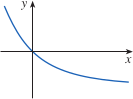
\includegraphics{img/img-0.png}
    \end{center}
    Yes.

\setcounter{enumi}{12}
    \item A function is given by a table of values, a graph, a formula, or a verbal description. Determine whether it is one-to-one.
    \[g(x) = 1 - \sin x\]
    No.

\setcounter{enumi}{16}
    \item Assume that f is a one-to-one function.
    \begin{enumerate}
        \item If $f(6) = 17$, what is $f^{-1}(17)$?
        \[f^{-1}(17) = 6\]
        \item If $f^{-1}(3) = 2$, what is $f(2)$?
        \[f(2) = 3\]
    \end{enumerate}
    \item If $f(x) = x^5 + x^3 + x$, find $f^{-1}(3)$ and $f(f^{-1}(2))$.\\
    Assume that $f(x)$ is a one-to-one function.
    \[x^5 + x^3 + x = 3\]
    \[x^5 + x^3 + x - 3 = 0\]
    \[x = 1\]
    Hence, $f^{-1}(3) = 1$.
    \[f(f^{-1}(2)) = 2\]

\setcounter{enumi}{23}
    \item Find a formula for the inverse of the function.
    \[h(x) = \frac{6-3x}{5x+7}\]
    Assume that $f(x)$ is a one-to-one function.
    \[y = \frac{6-3x}{5x+7}\]
    \[y(5x+7) = 6-3x\]
    \[5xy + 7y = 6 - 3x\]
    \[5xy + 3x = 6 - 7y\]
    \[x(5y+3) = 6 - 7y\]
    \[x = \frac{6-7y}{5y+3}\]
    Hence the inverse function is:
    \[f^{-1}(x) = \frac{6-7x}{5x+3}\]

\setcounter{enumi}{32}
    \item Use the given graph of $f$ to sketch the graph of $f^{-1}$.
    \begin{center}
        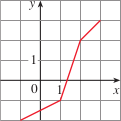
\includegraphics{img/img-1.png}
    \end{center}

\setcounter{enumi}{41}
    \item Find $(f^{-1})'(a)$.
    \[f(x) = x^3 + 3\sin x + 2 \cos x, a = 2\]
    \[(f^{-1})'(a) = \frac{1}{f'(x)}\text{, where } x \text{ satisfies } f(x) = 2\]
    \[x^3 + 3\sin x + 2 \cos x = 2\]
    \[x = 0\]
    Hence:
    \[(f^{-1})'(a) = \frac{1}{f'(0)} = \frac{1}{(x^3 + 3\sin x + 2\cos x)'} = \frac{1}{3x^2 + 3\cos x - 2\sin x}\]
    \[(f^{-1})'(a) = \frac{1}{3 \times 0^2 + 3\cos 0 - 2\sin 0} = \frac{1}{0 + 3 - 2} = \frac{1}{1} = 1\]

\setcounter{enumi}{46}
    \item If $f(x) = \int^x_3 \sqrt{1+t^3}dt$. Find $(f^{-1})'(0)$
    \[(f^{-1})'(0) = \frac{1}{f'(x)} \text{, where } x \text{ satisfies } f(x) = 0\]
    \[f(x) = 0\]
    \[\int^x_3 \sqrt{1+t^3}dt = 0\]
    \[x = 3\]
    By the Fundamental Theorem of Calculus:
    \[f'(x) = (\int^x_3 \sqrt{1+t^3}dt)' = \sqrt{1+x^3}\]
    \[(f^{-1})'(0) = \frac{1}{\sqrt{1 + 0^3}} = \frac{1}{1} = 1\]

\end{enumerate}

Section 6.2:

\begin{enumerate}
\setcounter{enumi}{1}
    \item Let:
    \begin{enumerate}
        \item How is the $e$ defined?\\
        $e$ is the number such that:
        \[lim_{h \to 0} \frac{e^h - 1}{h} = 1\]
        \item What is an approximate value for $e$?\\
        Approximate value of $e$ is: $2.71828$
        \item What is the natural exponential function?
        \[f(x) = e^x\]
    \end{enumerate}

\setcounter{enumi}{4}
        \item Graph the given functions on a common screen. How are these graphs related?
        \[y = 3^x \text{, } y = 10^x \text{, } y = (\frac{1}{3})^x \text{, }y = (\frac{1}{10})^x\]
        \begin{center}
            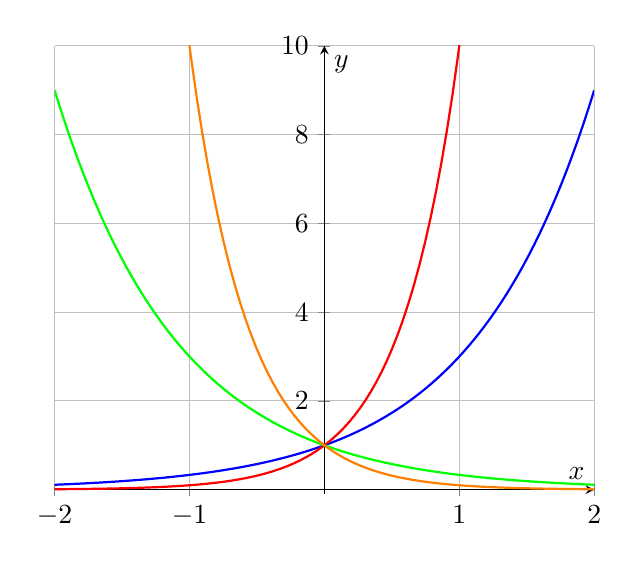
\begin{tikzpicture}
                \begin{axis}[
                    axis lines=middle,
                    xlabel={$x$},
                    ylabel={$y$},
                    xmin=-2, xmax=2,
                    ymin=-0.1, ymax=10,
                    legend pos=north west,
                    samples=100,
                    domain=-2:2,
                    grid=major,
                    legend style={font=\small}
                ]
                    % y = 3^x
                    \addplot[blue, thick] {3^x};
                    
                    % y = 10^x
                    \addplot[red, thick] {10^x};
                    
                    % y = (1/3)^x
                    \addplot[green, thick] {(1/3)^x};
                    
                    % y = (1/10)^x
                    \addplot[orange, thick] {(1/10)^x};
                \end{axis}
            \end{tikzpicture}
        \end{center}
        These graphs are symmentrical through the $y-axis$.

\setcounter{enumi}{10}
        \item Make a rough sketch by hand of the graph of the function.
        \[y = 1 - \frac{1}{2}e^{-x}\]
        \begin{center}
            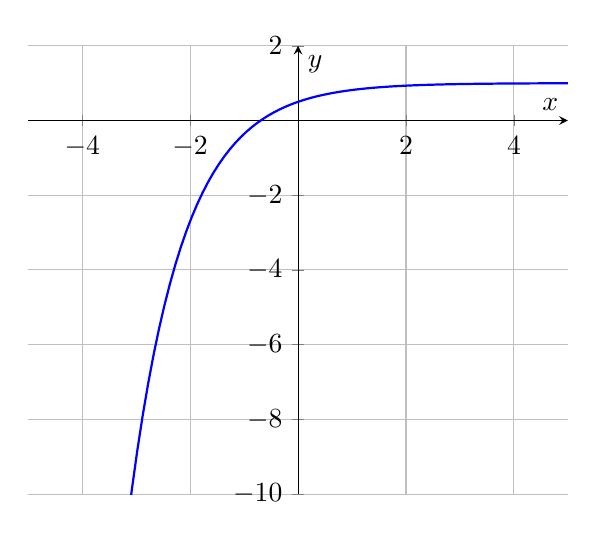
\begin{tikzpicture}
                \begin{axis}[
                    axis lines=middle,
                    xlabel={$x$},
                    ylabel={$y$},
                    xmin=-5, xmax=5,
                    ymin=-10, ymax=2,
                    legend pos=north west,
                    samples=100,
                    domain=-5:5,
                    grid=major,
                    legend style={font=\small}
                ]
                    % y = 1 - (1/2)e^-x
                    \addplot[blue, thick] {1 - (1/2)*exp(-x)};
                \end{axis}
            \end{tikzpicture}
        \end{center}

\setcounter{enumi}{12}
        \item Starting with the graph of $y = e^x$, write the equation of the graph that results from
        \begin{enumerate}
            \item shifting 2 units downward.
            \[y = e^x - 2\]
            \item shifting 2 units to the right.
            \[y = e^{x-2}\]
            \item reflecting about the $x-axis$.
            \[y = -e^{x}\]
            \item reflecting about the $y-axis$.
            \[y = e^{-x}\]
            \item reflecting about the $x-axis$ and then about the $y-axis$.
            \[y = -e^{-x}\]
        \end{enumerate}

\setcounter{enumi}{14}
        \item Find the domain of each function.
        \begin{enumerate}
            \item \(f(x) = \frac{1-e^{x^2}}{1-e^{1-x^2}}\)
            \[1-e^{1-x^2} \neq 0\]
            \[e^{1-x^2} \neq 1\]
            \[\log_e (e^{1-x^2}) \neq \log_e 1\]
            \[(1-x^2)\log_e(e) \neq 0\]
            \[x^2 \neq 1\]
            \[x \neq \pm 1\]
            Hence the domain of the function is: $(-\infty, \infty) \setminus \{-1,1\}$
            \item \(f(x) = \frac{1+x}{e^{\cos x}}\)
            \[e^{\cos x} \neq 0\]
            \[\log_e (e^{\cos x}) \neq \log_e 0\]
            Because $\log_e 0$ does not exist. Hence the domain of the function is $(-\infty,\infty)$
        \end{enumerate}
\setcounter{enumi}{19}
        \item Compare the functions $f(x) = x^5$ and $g(x) = 5^x$ by graphing both functions in several viewing rectangles. Find all points of intersection of the graphs correct to one decimal place. Which function grows more rapidly when $x$ is large?\\
        A small viewing rectangle with $x \in [-2,2]$ and $y \in [-20,20]$:
        \begin{center}
            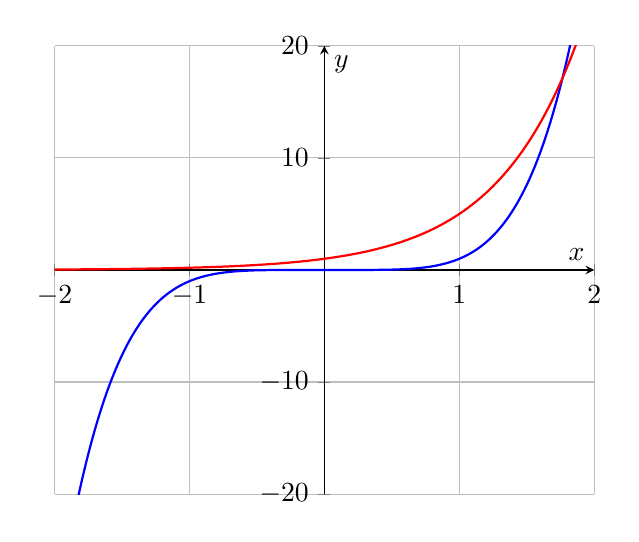
\begin{tikzpicture}
                \begin{axis}[
                    axis lines=middle,
                    xlabel=$x$, ylabel=$y$,
                    xmin=-2, xmax=2,
                    ymin=-20, ymax=20,
                    samples=100,
                    legend pos=north west,
                    grid=both,
                    minor grid style={gray!25},
                    major grid style={gray!50}
                ]
                    % Plot f(x) = x^5
                    \addplot[domain=-2:2, smooth, thick, blue] {x^5};
                    
                    % Plot g(x) = 5^x
                    \addplot[domain=-2:2, smooth, thick, red] {5^x};
                \end{axis}
            \end{tikzpicture}
        \end{center}
        A larger viewing rectangle with $x \in [-5,5]$ and $y \in [-300,300]$:
        \begin{center}
            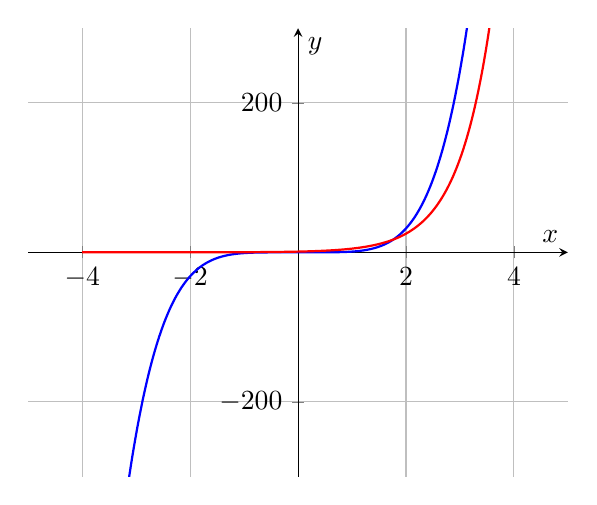
\begin{tikzpicture}
                \begin{axis}[
                    axis lines=middle,
                    xlabel=$x$, ylabel=$y$,
                    xmin=-5, xmax=5,
                    ymin=-300, ymax=300,
                    samples=100,
                    legend pos=north west,
                    grid=both,
                    minor grid style={gray!25},
                    major grid style={gray!50}
                ]
                    % Plot f(x) = x^5
                    \addplot[domain=-5:5, smooth, thick, blue] {x^5};
                    
                    % Plot g(x) = 5^x
                    \addplot[domain=-4:4, smooth, thick, red] {5^x};
                \end{axis}
            \end{tikzpicture}
        \end{center}
        There are two points of intersections which are approximately 1.8 and 5.\\
        The function $g(x) = 5^x$ grows more rapidly when $x$ is large.

\setcounter{enumi}{22}
        \item Find the limit:
        \[\lim_{x\to\infty}(1.001)^x = \infty\]
        Because $(1.001)^x$ will become infinitely larger as $x$ becomes infinitely larger.

\setcounter{enumi}{28}
        \item Find the limit:
        \[\lim_{x\to\infty}(e^{-2x}\cos x)\]
        Because $e^{-2x}$ will come closer to 0 as $x$ becomes larger and $\cos x$ only fluctuates between -1 and 1.\\
        Hence:
        \[\lim_{x\to\infty}(e^{-2x}\cos x) = 0\]

\setcounter{enumi}{32}
        \item Differentiate the function.
        \[f(x) = (3x^2-5x)e^x\]
        \[f'(x) = [(3x^2-5x)e^x]' = (3x^2-5x)'e^x + (e^x)'(3x^2-5x) = e^x(6x-5) + e^x(3x^2-5x)\]
        \[f'(x) = e^x(6x-5+3x^2-5x) = e^x(3x^2 + x - 5)\]
    
\setcounter{enumi}{38}
        \item Differentiate the function
        \[y = \sqrt[3]{e^x + 1}\]
        \[y = (e^x+1)^{1/3}\]
        \[y' = \frac{1}{3}(e^x+1)^{-2/3}e^x = \frac{e^x}{3}(e^x+1)^{-2/3}\]

\setcounter{enumi}{53}
        \item Find an equation of the tangent line to the curve $xe^y + ye^x = 1$ at the point (0,1).\\
        The slope of the tangent line is:
        \[(xe^y + ye^x)' = (1)'\]
        \[e^y + xe^y\frac{dy}{dx} + \frac{dy}{dx}e^x + ye^x = 0\]
        \[\frac{dy}{dx}(xe^y + e^x) = -e^y - ye^x\]
        \[\frac{dy}{dx} = \frac{-e^y - ye^x}{xe^y + e^x}\]
        \[\frac{dy}{dx}(0) = \frac{-e^1 - 1\times e^0}{0\times e^1 + e^0} = \frac{-e-1}{1} = -(e+1)\]
        Hence, the tangent line is:
        \[y = -x(e+1) + b\]
        Because the tangent line pass the point (0,1):
        \[1 = -0(e+1) + b\]
        \[b = 1\]
        Hence, the equation of the tangent line is:
        \[y = -x(e+1) + 1\]

\setcounter{enumi}{56}
        \item For what value of $r$ does the function $y = e^{rx}$ satisfy the differential equation:
        \[y'' + 6y' + 8y  = 0\]
        \[(e^{rx})'' + 6(e^{rx})' + 8(e^{rx}) = 0\]
        \[(re^{rx})' + 6re^{rx} + 8e^{rx} = 0\]
        \[r^2e^{rx} + 6re^{rx} + 8e^{rx} = 0\]
        Because $e^{rx}$ is not equal to 0 with every x:
        \[r^2 + 6r + 8 = 0\]
        \[r = -2 \text{ or } r = -4\]

\setcounter{enumi}{60}
        \item Let:
        \begin{enumerate}
            \item Use the Intermediate Value Theorem to show that there is a solution of the equation
            \[e^x + x = 0\]
            Let:
            \[f(x) = e^x + x\]
            This function is continuous with every $x$:\\
            Because of the IVT.\\
            Choose x = -1:
            \[f(-1) = e^{-1} - 1 = \frac{1}{e} - 1 < 0 \text{ Because $e > 1$.}\]
            Choose x = 1:
            \[f(1) = e^1 + 1 > 0 \text{ Because $e > 0$.}\]
            Hence, there is at least one solutions in the interval (-1,1).
        \end{enumerate}

\setcounter{enumi}{68}
        \item Find the absolute maximum value of the function $f(x) = x - e^x$.
        \[f'(x) = 1 - e^x = 0\]
        \[e^x = 1\]
        \[\log_e e^x = \log_e 1\]
        \[x = 0\]
        Hence, the absolute maximum value of the function is $f(0) = -1$.

\setcounter{enumi}{70}
        \item Find
        \[f(x) = xe^{2x}\]
        \begin{enumerate}
            \item the intervals of increase or decrease,
            \[f'(x) = e^{2x} + 2xe^{2x} = 0\]
            \[e^{2x} + 2xe^{2x} = 0\]
            \[e^{2x}(1 + 2x) = 0\]
            Because $e^{2x}$ will not be equal to 0 with every x.\\
            Hence:
            \[1 + 2x = 0\]
            \[x = -\frac{1}{2}\]
            Therefore, the function increases on the interval $(-\frac{1}{2}, \infty)$.\\
            The function decrease on the interval $(-\infty, -\frac{1}{2})$.
            \item the intervals of concavity, and
            \[f''(x) = 2e^{2x} + 2e^{2x} + 4xe^{2x} = 0\]
            \[4e^{2x} + 4xe^{2x} = 0\]
            \[4e^{2x}(1 + x) = 0\]
            Because $4e^{2x}$ will not equal 0 for every x.
            \[1 + x = 0\]
            \[x = -1\]
            Hence, the function concaves down on the interval $(-\infty, -1)$ and concaves up on the interval $(-1,\infty)$.
            \item the points of inflection.
            \[f(-1) = (-1)e^{-2} = -\frac{1}{e^2}\]
            Hence, the point of inflection is $(-1, -\frac{1}{e^2})$.
        \end{enumerate}

\setcounter{enumi}{80}
        \item Evaluate the integral.
        \[\int_0^1 (x^e + e^x) dx = (\frac{x^{e+1}}{e+1} + e^x)|_0^1 =  (\frac{1^{e+1}}{e+1} + e^1 - \frac{0^{e+1}}{e+1} - e^0) = \frac{1}{e+1} + e - 1 \]
        \[= \frac{1 + e^2 - 1}{e+1} = \frac{e^2}{e+1}\]

\setcounter{enumi}{83}
        \item Evaluate the integral.
        \[\int t^3e^{-t^4}dt\]
        Let:
        \[u = -t^4\]
        \[du = -4t^3dt\]
        \[-\frac{du}{4} = t^3dt\]
        \[-\frac{1}{4}\int e^{u}du = -\frac{1}{4}e^u + C = -\frac{1}{4}e^{-t^4} + C\]

\setcounter{enumi}{89}
        \item Evaluate the integral.
        \[\int e^{\sin \theta} \cos \theta \text{ } d\theta\]
        Let:
        \[u = \sin \theta\]
        \[du = \cos \theta d \theta\]
        \[\int e^u du = e^u + C = e^{\sin \theta} + C\]
\end{enumerate}

Section 6.3:

\begin{enumerate}
\setcounter{enumi}{2}
    \item Find the exact value of each expression.
    \begin{enumerate}
        \item \(\log_3 81\)
        \[\log_3 81 = 4\]
        \item \(\log_3 \frac{1}{81}\)
        \[\log_3 \frac{1}{81} = -4\]
        \item \(\log_9 3\)
        \[\log_9 3 = \frac{1}{2}\]
    \end{enumerate}

\setcounter{enumi}{4}
    \item Find the exact value of each expression.
    \begin{enumerate}
        \item \(\log_2 30 - \log_2 15\)
        \[\log_2 30 - \log_2 15 = \log_2 \frac{30}{15} = \log_2 2 = 1\]
        \item \(\log_3 10 - \log_3 5 - \log_3 18\)
        \[\log_3 10 - \log_3 5 - \log_3 18 = \log_3 \frac{10}{5} - \log_3 18 = \log_3 2 - \log_3 18\]
        \[ = \log_3 \frac{2}{18} = \log_3 \frac{1}{9} = -2\]
        \item \(2\log_5 100 - 4\log_5 50\)
        \[2\log_5 100 - 4\log_5 50 = \log_5 100^2 - \log_5 50^4 = \log_5 \frac{100^2}{50^4} = \log_5 \frac{10000}{6250000}\]
        \[= \log_5 \frac{1}{625} = -4\]
    \end{enumerate}

    \item Find the exact value of each expression.
    \begin{enumerate}
        \item \(e^{3\ln 2}\)
        \[e^{3\ln 2} = e^{\ln 2^3} = 2^3 = 8\]
        \item \(e^{-2\ln 5}\)
        \[e^{-2\ln 5} = e^{\ln 5^{-2}} = 5^{-2} = \frac{1}{25}\]
        \item \(e^{\ln (\ln e^3)}\)
        \[e^{\ln (\ln e^3)} = \ln e^3 = 3\ln e = 3\]
    \end{enumerate}

\setcounter{enumi}{7}
    \item Use the laws of logarithms to expand each expression
    \begin{enumerate}
        \item \(\ln \sqrt{\frac{3x}{x-3}}\)
        \[\ln \sqrt{\frac{3x}{x-3}} = \ln (\frac{3x}{x-3})^{1/2} = \frac{1}{2} \ln (\frac{3x}{x-3}) = \frac{1}{2} \ln 3x - \frac{1}{2} \ln (x-3)\]
        \item \(\log_2 [(x^3 + 1)\sqrt[3]{(x-3)^2}]\)
        \[\log_2 [(x^3 + 1)\sqrt[3]{(x-3)^2}] = \log_2 (x^3 + 1) + \log_2 \sqrt[3]{(x-3)^2} \]
        \[= \log_2 (x^3 + 1) + \log_2 (x-3)^{2/3} = \log_2 (x^3 + 1) + \frac{2}{3}\log_2 (x-3)\]
    \end{enumerate}

\setcounter{enumi}{9}
    \item Express as a single logarithm.
    \begin{enumerate}
        \item \(\ln 10 + 2\ln 5\)
        \[\ln 10 + 2\ln 5 = \ln 10 + \ln 5^2 = \ln (10 \times 5^2) = \ln (10 \times 25) = \ln 250\]
        \item \(\log_{10} 4 + \log_{10} a - \frac{1}{3} \log_{10} (a+1)\)
        \[\log_{10} 4 + \log_{10} a - \frac{1}{3} \log_{10} (a+1) = \log_{10} 4a - \log_{10} (a+1)^{1/3} = \log_{10} \frac{4a}{(a+1)^{1/3}}\]
    \end{enumerate}

\setcounter{enumi}{14}
    \item Use Formula 8 to graph the given functions on a common screen. How are these graphs related?
    \[y = \log_{1.5} x \text{, } y = \ln x \text{, } y = \log_{10} x \text{, } y = \log_{50} x\]
    \begin{center}
        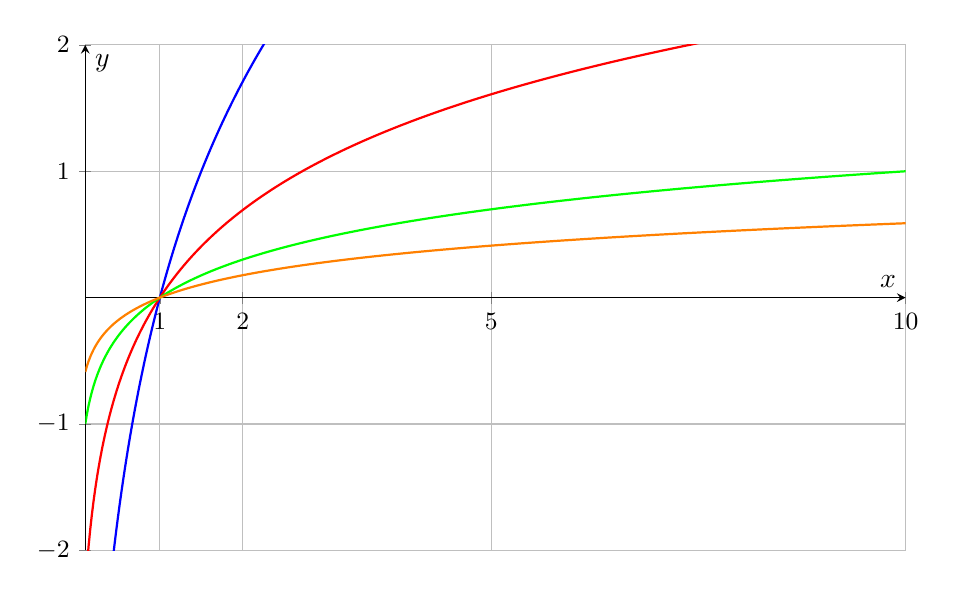
\begin{tikzpicture}
            \begin{axis}[
                width=12cm, height=8cm,
                xlabel={$x$},
                ylabel={$y$},
                xmin=0.1, xmax=10,
                ymin=-2, ymax=2,
                grid=major,
                legend style={at={(0.95,0.05)}, anchor=south east},
                axis lines=middle,
                xtick={1, 2, 5, 10},
                ytick={-2, -1, 0, 1, 2},
                ticklabel style={font=\small},
            ]
        
            % y = log_{1.5}(x)
            \addplot[
                domain=0.1:10,
                samples=500,
                thick,
                blue,
            ] {ln(x)/ln(1.5)};
        
            % y = ln(x)
            \addplot[
                domain=0.1:10,
                samples=500,
                thick,
                red,
            ] {ln(x)};
        
            % y = log_{10}(x)
            \addplot[
                domain=0.1:10,
                samples=500,
                thick,
                green,
            ] {ln(x)/ln(10)};
        
            % y = log_{50}(x)
            \addplot[
                domain=0.1:10,
                samples=500,
                thick,
                orange,
            ] {ln(x)/ln(50)};
        
            \end{axis}
        \end{tikzpicture}
    \end{center}
    All of these graphs are defined over $x > 0$.

\setcounter{enumi}{18}
    \item Make a rough sketch by hand of the graph of each function. Use the graphs given in Figures 2, and 3 and, if necessary, the transformations of Section 1.3.
    \begin{enumerate}
        \item \(y = \log_{10}(x+5)\)
        \item \(y = -\ln x\)
    \end{enumerate}
    \begin{center}
        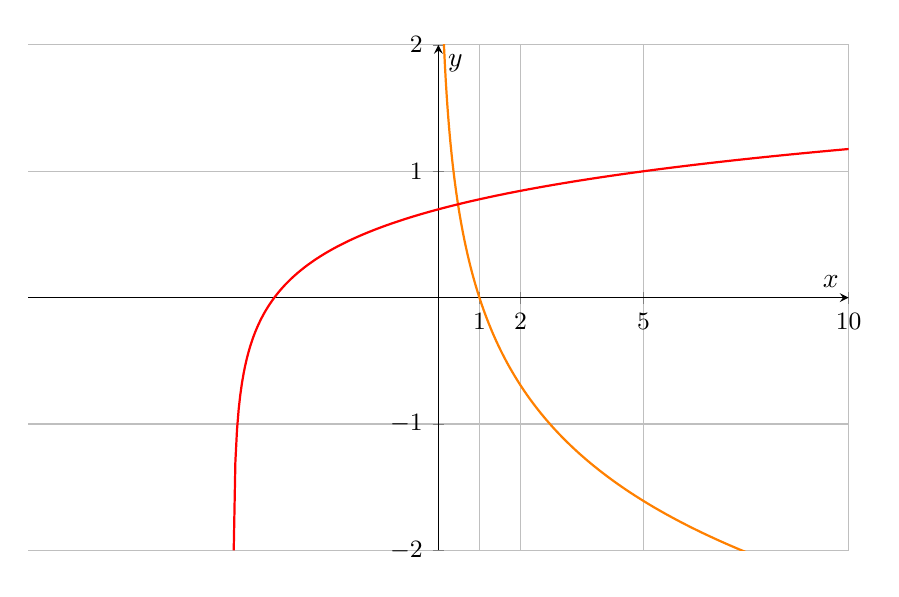
\begin{tikzpicture}
            \begin{axis}[
                width=12cm, height=8cm,
                xlabel={$x$},
                ylabel={$y$},
                xmin=-10, xmax=10,
                ymin=-2, ymax=2,
                grid=major,
                legend style={at={(0.95,0.05)}, anchor=south east},
                axis lines=middle,
                xtick={1, 2, 5, 10},
                ytick={-2, -1, 0, 1, 2},
                ticklabel style={font=\small},
            ]
            % y = log_{50}(x)
            \addplot[
                domain=0.1:10,
                samples=500,
                thick,
                orange,
            ] {-ln(x)};

            \addplot[
                domain=-10:10,
                samples=500,
                thick,
                red,
            ] {ln(x+5)/ln(10)};
        
            \end{axis}
        \end{tikzpicture}
    \end{center}

\setcounter{enumi}{21}
    \item Let:
    \[f(x) = \ln(x-1) - 1\]
    \begin{enumerate}
        \item What are the domain and range of $f$?
        \[x-1 > 0\]
        \[x > 1\]
        The domain of the function $f$ is $(1,\infty)$.\\
        The range of the function $f$ is $(-\infty, \infty)$.
        \item What is the $x$-intercept of the graph of $f$?
        \[\ln(x-1) - 1 = 0\]
        \[\ln(x-1) = 1\]
        \[x-1 = e\]
        \[x = e + 1\]
        Hence, the $x$-intercept of the graph $f$ is $e+1$.
        \item Sketch the graph of $f$.
        \begin{center}
            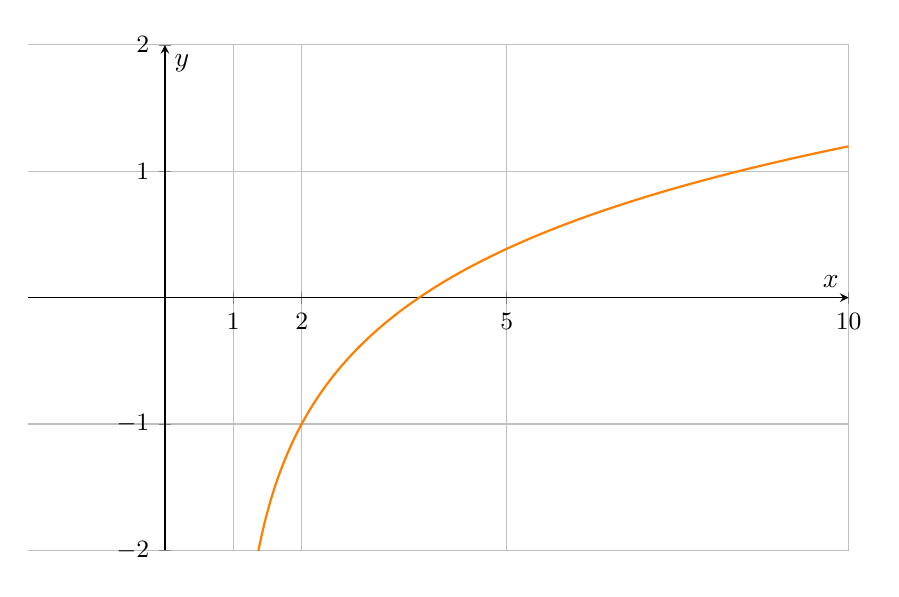
\begin{tikzpicture}
                \begin{axis}[
                    width=12cm, height=8cm,
                    xlabel={$x$},
                    ylabel={$y$},
                    xmin=-2, xmax=10,
                    ymin=-2, ymax=2,
                    grid=major,
                    legend style={at={(0.95,0.05)}, anchor=south east},
                    axis lines=middle,
                    xtick={1, 2, 5, 10},
                    ytick={-2, -1, 0, 1, 2},
                    ticklabel style={font=\small},
                ]
                % y = log_{50}(x)
                \addplot[
                    domain=0.1:10,
                    samples=500,
                    thick,
                    orange,
                ] {ln(x-1)-1};
                \end{axis}
            \end{tikzpicture}
        \end{center}
    \end{enumerate}

\setcounter{enumi}{24}
    \item Solve each equation for $x$. Give both an exact value and a decimal approximation, correct to three decimal places.
    \begin{enumerate}
        \item \(\ln x + \ln (x-1) = 0\)
        \[\ln x + \ln (x-1) = 0\]
        \[\ln (x-1) = - \ln x\]
        \[\ln(x-1) = \ln x^{-1}\]
        \[x - 1 = x^{-1}\]
        \[x - 1 = \frac{1}{x}\]
        \[x^2 - x - 1 = 0\]
        \[x = \frac{1+\sqrt{5}}{2} \approx 1.618 \text{ or } x = \frac{1-\sqrt{5}}{2} \approx -0.618\]
        Because $x > 1$ so that the equation can be defined.
        \[x = \frac{1+\sqrt{5}}{2} \approx 1.618\]
        \item \(5^{1-2x} = 9\)
        \[\log_5 5^{1-2x} = \log_5 9\]
        \[(1-2x)\log_5 5 = \log_5 9\]
        \[-2x = \log_5 (9) - 1 \]
        \[x = \frac{1 - \log_5 (9)}{2} \approx -0.183\]
    \end{enumerate}

\setcounter{enumi}{26}
    \item Find the limit.
    \[\lim_{x \to 2^+} e^{3/(2-x)} = 0\]

\setcounter{enumi}{30}  
    \item Differentiate the function.
    \[f(t) = -2e^t\]
    \[f'(t) = -2e^t\]

\setcounter{enumi}{40}
    \item Differentiate the function.
    \[y = x^2e^{-3x}\]
    \[y' = (x^2)'e^{-3x} + (e^{-3x})'(x^2)\]
    \[y' = 2xe^{-3x} - 3e^{-3x}x^2\]

\setcounter{enumi}{42}  
    \item Differentiate the function.
    \[f(t) = e^{at} \sin bt\]
    \[f'(t) = (e^{at})' \sin bt + e^{at} (\sin bt)'\]
    \[f'(t) = ae^{at} \sin bt + be^{at}\cos bt\]

\setcounter{enumi}{44}  
    \item Differentiate the function.
    \[F(t) = e^{t\sin 2t}\]
    \[F'(t) = e^{t\sin 2t}(t\sin 2t)'\]
    \[F'(t) = e^{t\sin 2t}(\sin 2t + 2t \cos 2t)\]

\setcounter{enumi}{48}  
    \item Differentiate the function.
    \[g(x) = \sin (\frac{e^x}{1+e^x})\]
    \[g'(x) = \cos (\frac{e^x}{1+e^x}) (\frac{e^x}{1+e^x})'\]
    \[g'(x) = \cos (\frac{e^x}{1+e^x})(\frac{(e^x)'(1+e^x) - (1+e^x)'e^x}{(1+e^x)^2})\]
    \[g'(x) = \cos (\frac{e^x}{1+e^x})(\frac{e^x(1+e^x) - e^{2x}}{(1+e^x)^2})\]
    \[g'(x) = \cos (\frac{e^x}{1+e^x})(\frac{e^x+e^{2x} - e^{2x}}{(1+e^x)^2})\]
    \[g'(x) = \cos (\frac{e^x}{1+e^x})(\frac{e^x}{(1+e^x)^2})\]

\setcounter{enumi}{54}
    \item Show that the function \(y = e^x + e^{-x/2}\) satisfies the differential equation \(2y'' - y' - y = 0\).
    \[y' = e^x - \frac{1}{2}e^{-x/2}\]
    \[y'' = e^x + \frac{1}{4}e^{-x/2}\]
    Hence:
    \[2y'' - y' - y = 2(e^x + \frac{1}{4}e^{-x/2}) - e^x + \frac{1}{2}e^{-x/2} - e^x - e^{-x/2}\]
    \[ = 2e^x + \frac{1}{2}e^{-x/2} - e^x + \frac{1}{2}e^{-x/2} - e^x - e^{-x/2} = 2e^x + e^{-x/2} - 2e^x - e^{-x/2} = 0\]


\end{enumerate}

\end{document}